%%%%%%%%%%%%%%%%%%%%%%%%%%%%%%%%%%%%%%%%%%%%%%%%%%%%%%%%%%%
% Chapter1


\pagestyle{fancy} 
\chapter{Background}
\label{cha:1}
\vspace{1cm}

\section{Variational Auto-Encoder (VAE) Structure}
\label{cha:VAE}
One of the reasons for which the generative models have been employed in different type of applications is the powerful and utility of VAE, where they are used to either solve issues in AI like image reconstruction and generation, achieve better results, reduce the computational complexity due to the high dimensionality of the data, find latent space, reduce dimensionality, extract and represent features or learn density distribution of the dataset. In this session it is given an overview on how a VAE network is structured and what are the main techniques applied to make it useful to each of the issues just mentioned.\\
Before starting to talk about the usage VAEs, it is mandatory to go through the structure of the auto-encoder which is essentially a neural network with a bottleneck in the middle Fig~\ref{fig:autoencoder} designed to reconstruct the original input in an unsupervised way, in other words, it learns an identity function by first reducing the dimension of the data to the bottleneck so as to extract more efficient and compressed representation. Surprisingly The idea was originated in the 1980s, and later promoted by the seminal paper by~\cite{hinton2006reducing}.

\vspace{0.3cm}
The Auto-Encoder consists of tow connected networks that could be any kind of neural networks (convolutional, or multi-layer perceptron etc) depends on the data it has to deal with, which are:
\begin{itemize}
	\item Encoder network: gets the high-dimension input and transform it to into a low-dimension code in the bottleneck, or we can call it representation, latent or features as well again depends on what the usage are we making of the auto-encoder.
	\item Decoder network: gets the output of the encoder and does essentially the inverse process, or we can say reconstruct the data, likely with larger and larger layers to the last one that outputs the reconstructed original data.
\end{itemize}

\begin{figure}
	\centerline
	\autoencoder
	\caption{Autoencoder}
	\label{fig:autoencoder}
\end{figure} 

We can see already how the auto-encoder networks can give us an efficient way to  impressively represent the data and in lower dimension. So the accomplishment of solutions for the problematics we talked about at beginning of this session, is all about about how we build the bottleneck layer or what will call from now on vector $z$. The VAE~\cite{kingma2013auto} basically is an auto-encoder but the structure of vector $z$ is quite different. For instance what if we need to map the input into a probability distribution $q_{\theta}$ instead of a fixed vector $z$, where $q_{\theta}$ is parameterized by $\theta$, from which we sample or generate $z$, this is what make the VAE to be recognized as a generative model. Where the training is regularized to avoid eventual overfitting  that might occur with auto-encoder architecture and ensure that the distribution $q_{\theta}$ has good parameters to enable the generative process. The way that makes the encoder to be able to produce $q_\theta$ is by composing the bottleneck or the output of a mean $\mu$ and a covariance matrix $\Sigma$ the problem here is that nothing would prevent the this distribution to be extremely narrow, or effectively a single value. To escape the issue, the Kullback-Leibler (KL) divergence-which measures the distance between tow distributions- is introduced  between the distribution produced by the encoder $q_{\theta}(z \mid x_i)$ and a unit Gaussian distribution $p(z)$(mean $0$, covariance matrix is the identity matrix) and tell us how much information is lost when using q to represent p, this KL divergence is then introduced as a penalty to the loss function li, which consists of another term as well that is the expected negative likelihood of the $i$-th datapoint $x_i$ as follow:


\begin{equation}
l_i(\theta,\phi)=-E_{z\sim q_\theta (z\mid x_i)}[\log_{p_\phi}(x_i \mid z)]+KL(q_\theta (z\mid x_i)||p(z))
\label{eq:VAE_loss}
\end{equation}
Where $z$ is sampled from $q_\theta$ and $\phi$ the decoder parameters, the purpose of the first term in poor words mean \textacutedbl how much the decoder output is similar to original datapoint $x_i$\textgravedbl. It intuitively leads the decoder to learn to reconstruct the data. The last important part left to talk about is the training one, we can use the gradient descent to optimize the loss with respect to the parameters of the encoder and decoder $\theta$ and $\phi$ respectively. For stochastic gradient descent with step size $\rho$, the encoder parameters are updated using $\theta=\theta-\frac{\partial l}{\partial \theta} $  and the decoder is updated similarly.



\subsection{Reparameterization Trick:}
\label{cha:VAE_REparam}
As we can notice at this point that there would be a problem doing the backpropagation step of the gradient descent optimizer, because it does not go through the random node z, therefore we have to implement some trick to circumvent this issue. The reparameterization trick~\cite{kingma2013auto} is essentially done by introducing an auxiliary variable (noise) $\varepsilon$ that allows us to reparameterize $z$ in a way that allows backpropagate to flow through the deterministic nodes as shown in Fig.~\ref{fig:paratrick}, we are basically expressing the random variable $z$ as a deterministic 

\begin{figure}
	\centerline
	\paratrick
	\caption{reparameterization trick}
	\label{fig:paratrick}
\end{figure} 

\section{Gaussian Mixture Models (GMMs) structure and learning algorithm}

\label{cha:GMM}
GMM is a probabilistic model for representing normally distributed subpopulations within an overall population. Mixture models in general don't require knowing which subpopulation a data point belongs to, allowing the model to learn the subpopulations automatically. Since subpopulation assignment is not known, this constitutes a form of unsupervised learning. GMMs have been used for feature extraction from speech data, and have also been used extensively in object tracking of multiple objects, where the number of mixture components and their means predict object locations at each frame in a video sequence.
The model is parameterized by two types of values, the mixture component weights are defined as $\theta_k$ and the component means $\mu_k$ and variances $\sigma_k$ or covariances (for the multivariant case) $\Sigma$, the mixture component weights has a constraint that is:  $\sum_{i=1}^{K} \phi_i = 1$ so that the total probability distribution normalizes to 1. The numerical technique used to maximize the likelihood estimation is the Estimation maximization (EM) which consists of tow steps:

\begin{itemize}
	\item	 E-step: consist of calculating the the expectation of the component assignments $P(C_k | x_i)$ for each data point $x_i \in X$ given the model parameters $\phi_k$,  $\mu_k$, and $\sigma_k$.
\end{itemize}
\begin{itemize}
	\item	M-step: which consists of maximizing the expectations calculated in the E step with respect to the model parameters. This step consists of updating the values $\phi_k$,  $\mu_k$, and $\sigma_k$.
\end{itemize}
The entire process iteratively repeats until the algorithm converges, before it starts some initializations are made as follows:
Randomly assign samples without replacement from the dataset $X={x_1, ..., x_N}$, to the component mean estimates $\mu_1,..., \mu_k$. E.g. for K=3 and N=100, set $\mu_1= x_{45}$, $\mu_2 = x_{32}$, $\mu_3 = x_{10}$. 
Set all component variance estimates to the sample variance 
$\sigma_1^2,...,\sigma_k^2=\frac{1}{N}\sum_{i=1}^{K} (x_i -\hat{x})^{2}=1$, where $\hat{x}=\frac{1}{N}\sum_{i=1}^{N}(x_i)$ is the sample mean.
Set all component distribution prior estimates to the uniform distribution  
$P(C_k) = \phi_1,..., \phi_k  = \frac{1}{K}$
while the E-step computes the probability that $x_i$ is generated by component $C_k$:
\begin{equation}
p(C_j \mid x_i ) = \frac{ p(x_i \mid C_j)p(C_j) }{p(x_i)} = \frac{p(x_i \mid C_j)p(C_j)}{\sum_ip(x_i \mid C_j)p(C_j)}
\label{eq:}	
\end{equation}

which will be used in the M-step where the parameters are updated as follow:	

\begin{align}
\mu_j&=\frac{ \sum_{i} p(C_j \mid x_i )x_i}{\sum_{i} {p(C_j \mid x_i )}} \\
\sigma_j^2 &=\frac{\sum_{i}{p ( C_j \mid x_i)}  (x_i - \mu_j) (x_i - \mu_j)^T} {\sum_{i} {p(C_j \mid x_i )}} \\
p ( C_j ) &= \frac{ \sum_{i} p(C_j \mid x_i )}{N}
\end{align}

\begin{figure}
	\centering
	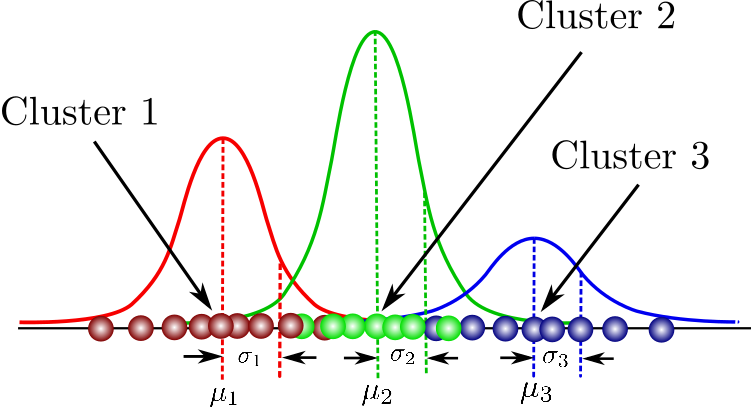
\includegraphics[scale=0.3]{Figures/GMM}
	\caption{}
	\label{fig:GMM}
\end{figure}

\vspace{10pt} 
Originally GMM is employed for classification and clustering tasks, but as we can deduce that it is also a suitable model when recovering the distribution of the data is needed, since it can produce more complexed distribution composed of jointed k gaussians as in Fig.~\ref{fig:GMM}, for example if we have different sources from which the data is provided. Back to our main argument, GMM has been used in several robotics applications, like in Gaussian Mixture Model for Robotic Policy Imitation~\cite{pignat2019bayesian} where different robots had to learn from few amount of demonstrations to complete various tasks such as avoid obstacles, or insert a peg in a moving hole. This approach (GMM) illustrates the advantages of learning a distribution of policies instead of trajectories and can be used in a variety of tasks. On the other hand in some work as in~\cite{zhang2016robot} the GMM was benefited in robot obstacle avoidance learning as a base for a generative model, to generate trajectories, by Gaussian Mixture Regression (GMR), The trajectory obtained not only can avoid obstacles but also can be executed by robots due to its good smooth property. The same idea of~\cite{zhang2016robot} was implemented in~\cite{reiley2010motion} in which GMM encodes the expert\textquotesingle s underlying motion structure. GMR is then used to extract a smooth reference trajectory to reproduce a trajectory of the task. This GMM/GMR generative model was trained on expert data, then tested by classifying the generated trajectories  to be either coming from expert, intermediate, or novice surgeons. The classification algorithm Hidden Markov Models (HMMs) trains three (expert, intermediate and novice) from five new unseen trials for each skill level. The results of the classifier show that each trajectories generated by GMM/GMR are closest to the expert model. To conclude this session it is right and proper to say that the use of GMM has remarkable impact to improve the model performance in presence of lack of data issue.


%\vspace{1cm}
\section{Reinforcement Learning RL}

\label{cha:RL}
This field of machine learning deals with how an agent ought to behave in an environment in order to maximize the reward. It differs from supervised learning in not needing of labeled input/output pairs and from unsupervised learning in getting guidance from the environment by performing actions and learning from the errors or rewards. Typically the environment takes the form of a Markov Decision Process (MDP) is a mathematical system used for modeling decision making. We use a tuple $(S, A, P, R, \gamma)$ to define a MDP. Where $S$ denotes the state space, a finite set of states. $A$ denotes a set of actions the actor can take at each time step $t$. $P$ denotes the probability that taking action a at time step $t$ in state $s_t$ will result in state $s_{t+1}$. $R_a(s,\acute{s})$ is the expected reward from taking action a and transitioning to $\acute{s}$. $\gamma \in [0, 1]$ is a discount factor, to discount the future reward. The general diagram of Reinforcement learning is shown in Fig.~\ref{fig:RL}
\begin{figure}
	\centerline
	\RL
	\caption{Reinforcement learning diagram}
	\label{fig:RL}
\end{figure} 
\vspace{0.3cm}
There are tow notions about the environment where the algorithm that implement RL that should be mentioned which are:
\begin{itemize}
	\item \textacutedbl model-based\textacutedbl algorithms: who are employed when the environment is a priori known, in other words, when we know the transition probability matrix P between states, so the agent can make predictions about the next state and reward before it takes each action.
\end{itemize}
\begin{itemize}
	\item \textacutedbl model-free\textacutedbl algorithms: for which there is no assumption about the world.
\end{itemize}
While about the techniques the algorithm uses to lean the policy are divided as follow:
\begin{itemize}
	\item \textquotedblleft Off-policy\textquotedblright: is that it updates its Q-values using the Q-value of the next state s\textasciigrave and the greedy action a\textasciigrave. In other words, it estimates the return (total discounted future reward) for state-action pairs assuming a greedy policy were followed despite the fact that it is not following a greedy policy.
\end{itemize}
\begin{itemize}
	\item \textquotedblleft On-policy\textquotedblright: is that it updates its Q-values using the Q-value of the next state s\textasciigrave and the current policy\textasciigrave{s} action a. It estimates the return for state-action pairs assuming the current policy continues to be followed.
\end{itemize}

In this work, all the algorithms referred to are model-free since in robotics applications usually the software agent can not make any prediction about the environment, and no assumption is made whether it is on-policy or off-policy.

\vspace{0.3cm}
Going through the various algorithms of RL you can realize that in most cases there is not best algorithm, it all depends on task, environment, discrete or continuous spaces, and the data itself and its size. During my studies I have implemented different algorithms in RL which are Deep Q Learning (DQN), Deep Deterministic Policy Gradient (DDPG) and Trust Region Policy Optimization (TRPO). Basing on my modest experience I realized is that as long as we have simple and well-defined environment, picking the algorithm who is more fit to the task taking into account the domain spaces of actions and states, eventually will get good results, the agent will learn a close-to-optimal policy to behave in the environment. But when the task (policy) to be learned is more complicated in respect of the lack of resources and data and its quality, then it is more than convenient making some process on the input data to make the learning policy process more efficient computationally and of course in terms of results which are our aim first of all, for example find the latent space of the data, or define a probability distribution that describe the dataset. That what I found out while doing my survey about generative models in robotics, where RL is strongly present regardless on which algorithm has been employed, actually most of times the algorithm used was not mentioned. 

\section{Generative Adversarial Networks (GANs)}

\label{cha:GANs}
Generative adversarial networks (GAN) is algorithmic architecture that uses two neural networks, pitting one against the other (thus the \textacutedbl adversarial\textgravedbl) in order to generate new, synthetic instances of data that can pass for real data. They are used widely in image generation, video generation and voice generation. it was introduced firstly by~\cite{goodfellow2014generative} to create a new framework for estimating generative models via an adversarial process that corresponds to tow-player game,
the tow networks could have arbitrary architecture and they are trained simultaneously, one neural network, called the discriminator, is designed as classifier network to evaluate the authenticity  distinguishing between fake and real data instances, while the other one, called generator, is trained to generate data as close to the authentic ones. Meanwhile, the generator is creating new, synthetic instances that it passes to the discriminator. It does so in the hopes that they, too, will be deemed authentic, even though they are fake. The goal of the generator is to generate passable instances to lie without being caught. The goal of the discriminator is to identify those coming from the generator as fake. GANs are a clever way to train a generative model in the same manner of a supervised learning problem.\\
To describe the GAN algorithm Fig.~\ref{fig:GAN} it is possible to start from either the generator, or the discriminator, because as mentioned in the previous section it corresponds to a tow-player game, like in chess, conventionally the while starts, but even if black starts that does not change the essence of the game. However, let's start with the more interesting one with is the generative model.\\
\begin{figure}
	\centerline
	\GAN
	\caption{GAN Architecture}
	\label{fig:GAN}
\end{figure} 
The generator model takes a fixed-length random noise vector as input and generates a sample in the domain. The vector is drawn randomly from a Gaussian distribution, and the vector is used to seed the generative process. This vector space is referred to as a latent space, or a vector space comprised of latent variables. Latent variables, or hidden variables, are those variables that are important for a domain but are not directly observable. It is often referred to latent variables, or a latent space, as a projection or compression of a data distribution. That is, a latent space provides a compression or high-level concepts of the observed raw data such as the input data distribution. In the case of GANs, the generator model applies meaning to points in a chosen latent space, such that new points drawn from the latent space can be provided to the generator model as input and used to generate new and different output examples, 
after training, the generator model is kept and used to generate new samples. Sometimes, the generator can be repurposed as it has learned to effectively extract features from examples in the problem domain. Some or all of the feature extraction layers can be used in transfer learning applications using the same or similar input data. \\

The Discriminator Model takes an example from the domain as input (real or generated) and predicts a binary class label of real or fake (generated).The real example comes from the training dataset. The generated examples are output by the generator model. The discriminator is a normal (and well understood) classification model. After the training process, the discriminator model is discarded as we are interested in the generator.\\
The generator and the discriminator have different training processes, and it proceeds in alternating periods:
\begin{enumerate}
	\item The discriminator trains for one or more epochs.
	\item The generator trains for one or more epochs.
	\item Repeat steps 1 and 2 to continue to train the generator and discriminator networks.
\end{enumerate}

Indeed, as the generator improves with training, the discriminator get worse, because it becomes more difficult to recognize the authentic instances rather than the generated one, which means in accuracy terms that if the generator succeeds perfectly then the discriminator has a 50\% accuracy, same as flipping a coin to predict the label of the current instance.
This progression poses a problem for convergence of the GAN as a whole: the discriminator feedback gets less meaningful over time. If the GAN continues training past the point when the discriminator is giving completely random feedback, then the generator starts to train on junk feedback, and its own quality may collapse, which produces limited varieties of samples. Contrarily. If the discriminator gets too successful that the generator gradient vanishes and learns nothing.
Anyways, training GANs is noted as hard to obtain but still there several techniques to make the training more stable, which are out of the boundaries of this work. GANs try to replicate a probability distribution. They should therefore use loss functions that reflect the distance between the distribution of the data generated by the GAN and the distribution of the real data. Of course, there are tow loss functions for each of the tow networks as introduced in~\cite{goodfellow2014generative}, the generator tries to minimize the following function while the discriminator tries to maximize it:
\begin{equation}
E_x[\log{D(x)}] + E_z[\log{(1-D(G(z)))}]
\label{eq:GAN_loss}
\end{equation}

where $D(x)$ is the discriminator's estimate of the probability that real data instance x is real.
$E_x$ is the expected value over all real data instances. $G(z)$ is the generator's output when given noise z. $D(G(z))$ is the discriminator's estimate of the probability that a fake instance is real.
$E_z$ is the expected value over all random inputs to the generator (in effect, the expected value over all generated fake instances $G(z)$). The formula derives from the cross-entropy between the real and generated distributions. Since the generator can not directly affect $\log{D(x)}$ so, for the generator, minimizing the loss is equivalent to minimizing $log(1 - D(G(z)))$.


\clearpage{\pagestyle{empty}\cleardoublepage}